\chapter{Differential equations with inputs}
\section{RC with exponential input}
\begin{figure}
  \centering
  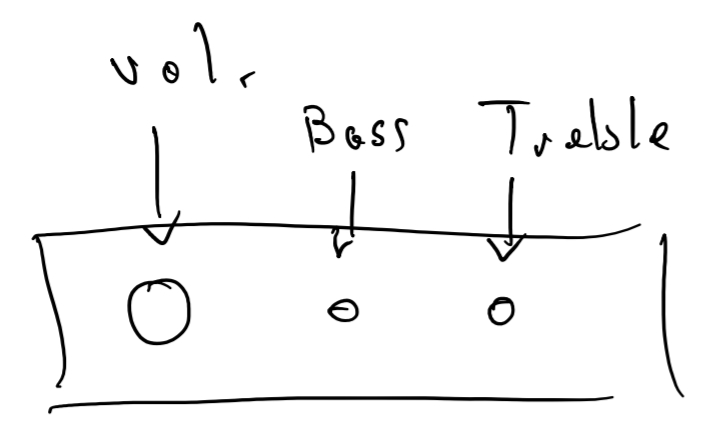
\includegraphics[width=0.5\linewidth]{figures/4/amp}
  \caption{An amp with three knobs to adjust playback.}
  \label{figure:lec4-amp}
\end{figure}
\begin{figure}
  \centering
  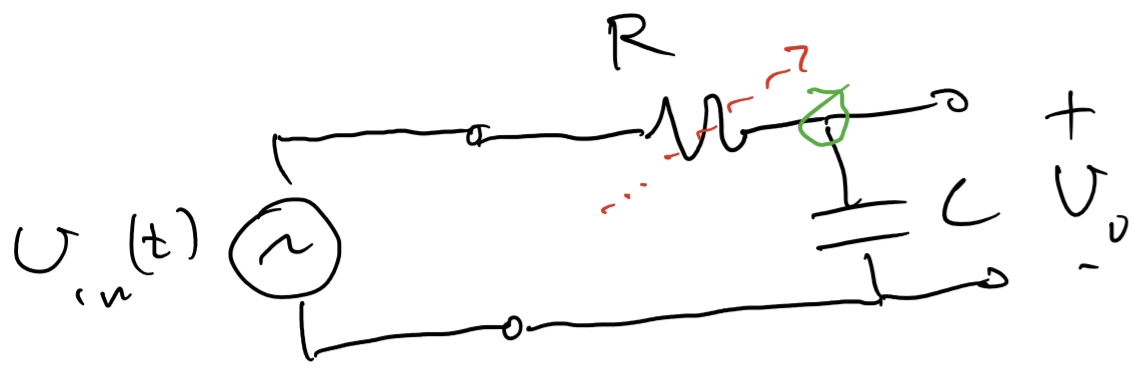
\includegraphics[width=1\linewidth]{figures/4/RC}
  \caption{RC circuit as a filter.}
  \label{figure:lec4-RC}
\end{figure}

In this section we will derive, in a more hands-on way, the behavior of an RC circuit forced by an exponential input.
If you have ever used an amp%
% \footnote{Specifically, a less-cool solid-state one.}
with knobs for treble and bass (\autoref{figure:lec4-amp}), then you have interacted with two circuits
similar to the one shown in \autoref{figure:lec4-RC}.
The resistor with a arrow is a variable resistor, or potentiometer,%
\footnote{Electric guitars use this circuit component, which guitarists call ``pots,'' to blend the pickups' signals.}
that might be controlled by one of the amp's knobs.

In \autoref{figure:lec4-RC},
\begin{itemize}
  \item \(v_\text{in}\) represents the amp's analog input,
  \item \(v_o\) is used to drive the speakers after subsequent amplification, and
  \item \(R\) represents the setting on one of the potentiometers.
\end{itemize}
By studying the distinguished (green) node, we can write the following differential equation:
\begin{align}
  \label{eqn:lec4-RC}
  \dod{}{t} v_o(t)
  &= -\frac{1}{RC} v_o(t) + \frac{1}{RC} v_\text{in}(t).
  \intertext{We'll constrain \(v_\text{in}\) to have the following form:}
  v_\text{in}(t)
  &= V_\text{in} e^{st}.
  \intertext{While it seems that this form is arbitrary, it will prove  insightful, because \(e^{st}\) is an \emph{eigenfunction} for input-output behavior of this circuit, i.e.\ we expect}
  v_o(t) &= V_o e^{st}.
  \intertext{We can determine \(V_o\) by substituting our parameterization of \(v_o\) into \autoref{eqn:lec4-RC}, whose LHS\ldots}
  \dod{}{t} v_o(t)
  &= \dod{}{t} V_o e^{st} \\
  &= sV_o e^{st}
  \intertext{\ldots is equated with the RHS:}
  sV_o e^{st}
  &= -\frac{1}{RC} V_o e^{st} + \frac{1}{RC} V_\text{in} e^{st}.
  \intertext{Now we can isolate \(V_o\).}
  sV_0 + \frac{1}{RC} V_o
  &= \frac{1}{RC} V_\text{in} \\
  V_o
  &= \del{\frac{1}{RC}} \del{\frac{1}{s + \frac{1}{RC}}} V_\text{in}
  \intertext{Substituting \(\lambda = -\frac{1}{RC}\),}
  V_o
  &= \frac{1}{1 - \frac{s}{\lambda}} V_\text{in}
  \intertext{All together, our solution for \(v_o(t)\) is the following:}
  v_o(t) = V_o e^{st}
  &= \frac{1}{1 - \frac{s}{\lambda}} V_\text{in} e^{st}.
  \intertext{Suppose that we have an initial condition for \(v_o\) at time 0.}
  \eval{ v_o }_{t = 0}
  &= v_1
  \intertext{Then our solution, taking this fact into account, will be}
  v_o(t) &= A e^{-\frac{t}{RC}} +
  \frac{1}{RC}
    \del{\frac{V_\text{in} e^{st}}{s + \frac{1}{RC}}},
  \intertext{where \(A\) remains to be determined, viz.\ by evaluating both sides at \(t = 0\):}
  v_1 &= A + \frac{1}{RC} \del{\frac{V_\text{in}}{s + \frac{1}{RC}}}\\
  A &= v_1 - \frac{1}{RC} \del{\frac{V_\text{in}}{s + \frac{1}{RC}}}.
  \intertext{This concludes our example. A solution to a linear differential equation will, generally, have the following structure:}
  v(t)
  &= v_\text{homogeneous}(t) + v_\text{particular}(t),
  \intertext{where \(v_\text{homogeneous}(t)\) corresponds to the initial condition, and \(v_\text{particular}(t)\) to the input term.}
\end{align}

\section{General scalar differential equation}
We will verify that the following general differential equation:
\begin{align}
  \label{eqn:lec4-general-diffeq}
  \dod{}{t} x(t)
  &= \lambda x(t) + u(t); \quad x(t_0) = x_0
  \intertext{has the following solution, which is a sum of a homogeneous and a particular term:}
  x(t)
  &= e^{\lambda(t - t_0)} x_0
  + \int_{t_0}^t e^{\lambda (t - \tau)} u(\tau) \dif \tau.
  \intertext{We can check the initial condition \(x(t_0) = x_0\): the former term evaluates to \(x_0\) and the latter to \(0\).
  Next, we can verify that
  \(\od{}{t} x(t)
  = \lambda x(t) + u(t)\) holds by differentiating.}
  \dod{}{t} x(t)
  &= \bigg\{ \lambda e^{\lambda (t - t_0)}
             x_0
           \bigg\} +
  u(t) +
  \bigg\{
    \int_{t_0}^{t} \lambda e^{\lambda (t - \tau) } u(\tau) \dif \tau
  \bigg\}
\end{align}
% (The latter two terms result from Leibniz's rule for differenting definite integrals.)
The two terms in curly braces sum to \(\lambda x(t)\), so \autoref{eqn:lec4-general-diffeq} is satisfied.
